\documentclass{report}
% Include all project wide packages here.
\usepackage{fullpage}
\usepackage[style=ieee]{biblatex}
\usepackage[dutch]{babel}

\renewcommand{\familydefault}{\sfdefault}

\setmainfont[Ligatures=TeX]{Myriad Pro}
\setmathfont{Asana Math}
\setmonofont{Lucida Console}

\usepackage{titlesec, blindtext, color}
\definecolor{gray75}{gray}{0.75}
\newcommand{\hsp}{\hspace{20pt}}
\titleformat{\chapter}[hang]{\Huge\bfseries}{\thechapter\hsp\textcolor{gray75}{|}\hsp}{0pt}{\Huge\bfseries}
\renewcommand{\familydefault}{\sfdefault}
\renewcommand{\arraystretch}{1.2}
\setlength\parindent{0pt}

%For code listings
\definecolor{black}{rgb}{0,0,0}
\definecolor{browntags}{rgb}{0.65,0.1,0.1}
\definecolor{bluestrings}{rgb}{0,0,1}
\definecolor{graycomments}{rgb}{0.4,0.4,0.4}
\definecolor{redkeywords}{rgb}{1,0,0}
\definecolor{bluekeywords}{rgb}{0.13,0.13,0.8}
\definecolor{greencomments}{rgb}{0,0.5,0}
\definecolor{redstrings}{rgb}{0.9,0,0}
\definecolor{purpleidentifiers}{rgb}{0.01,0,0.01}


\lstdefinestyle{csharp}{
language=[Sharp]C,
showspaces=false,
showtabs=false,
breaklines=true,
showstringspaces=false,
breakatwhitespace=true,
escapeinside={(*@}{@*)},
columns=fullflexible,
commentstyle=\color{greencomments},
keywordstyle=\color{bluekeywords}\bfseries,
stringstyle=\color{redstrings},
identifierstyle=\color{purpleidentifiers},
basicstyle=\ttfamily\small}

\lstdefinestyle{c}{
language=C,
showspaces=false,
showtabs=false,
breaklines=true,
showstringspaces=false,
breakatwhitespace=true,
escapeinside={(*@}{@*)},
columns=fullflexible,
commentstyle=\color{greencomments},
keywordstyle=\color{bluekeywords}\bfseries,
stringstyle=\color{bluestrings},
identifierstyle=\color{purpleidentifiers}
}

\lstdefinestyle{vhdl}{
language=VHDL,
showspaces=false,
showtabs=false,
breaklines=true,
showstringspaces=false,
breakatwhitespace=true,
escapeinside={(*@}{@*)},
columns=fullflexible,
commentstyle=\color{greencomments},
keywordstyle=\color{bluekeywords}\bfseries,
stringstyle=\color{redstrings},
identifierstyle=\color{purpleidentifiers}
}

\lstdefinestyle{xaml}{
language=XML,
showspaces=false,
showtabs=false,
breaklines=true,
showstringspaces=false,
breakatwhitespace=true,
escapeinside={(*@}{@*)},
columns=fullflexible,
commentstyle=\color{greencomments},
keywordstyle=\color{redkeywords},
stringstyle=\color{bluestrings},
tagstyle=\color{browntags},
morestring=[b]",
  morecomment=[s]{<?}{?>},
  morekeywords={xmlns,version,typex:AsyncRecords,x:Arguments,x:Boolean,x:Byte,x:Char,x:Class,x:ClassAttributes,x:ClassModifier,x:Code,x:ConnectionId,x:Decimal,x:Double,x:FactoryMethod,x:FieldModifier,x:Int16,x:Int32,x:Int64,x:Key,x:Members,x:Name,x:Object,x:Property,x:Shared,x:Single,x:String,x:Subclass,x:SynchronousMode,x:TimeSpan,x:TypeArguments,x:Uid,x:Uri,x:XData,Grid.Column,Grid.ColumnSpan,Click,ClipToBounds,Content,DropDownOpened,FontSize,Foreground,Header,Height,HorizontalAlignment,HorizontalContentAlignment,IsCancel,IsDefault,IsEnabled,IsSelected,Margin,MinHeight,MinWidth,Padding,SnapsToDevicePixels,Target,TextWrapping,Title,VerticalAlignment,VerticalContentAlignment,Width,WindowStartupLocation,Binding,Mode,OneWay,xmlns:x}
}

%defaults
\lstset{
basicstyle=\ttfamily\small,
extendedchars=false,
numbers=left,
numberstyle=\ttfamily\tiny,
stepnumber=1,
tabsize=4,
numbersep=5pt
}
\addbibresource{../../library/bibliography.bib}

\title{EPO-2: Mid-term Design Report - Director}
\author{}

\begin{document}

\chapter{Director}
\label{ch:director}
Het programma wat voor de besturing van de robot zorgt op de computer, door ons ``Director'' gedoopt, bestaat zoals eerst beschreven uit vier hoofdonderdelen. De laatste drie worden hier beschreven. We kunnen hiervoor de volgende eisen opstellen:

\section{Eisen}
\begin{itemize}
\item De pathfinder op basis van het A* algoritme
\item De event-driven seriële implementatie
\item De controller
\item De gebruikersinterface en visualisatie
\end{itemize}

\section{Ontwerp en Implementatie}
\label{sec:dirImplementatie}
We hebben uiteindelijk, zoals te lezen is in hoofdstuk \ref{ch:route}, gekozen voor een routeplanner gebaseerd op A*. Deze compileren we naar een standaard C dll (stdcall).

Ons hoofdproject wordt geschreven in C\# (.NET 4.5) en in combinatie met Windows Presentation Foundation of WPF, een UI framework waarin de gebruikers interface beschreven wordt in XAML (Extensible Application Markup Language).
XAML is een taal die heel erg lijkt op XML.
Dit geeft een vriendelijkere ontwikkelomgeving, managed talen zijn nu eenmaal wat vriendelijker voor de programmeur.
Het hebben van een UI oogt prettiger en het gebruik van het eventmodel is heel fijn voor de seriële communicatie.
Dit heeft deels met persoonlijke voorkeur te maken, maar om de code voor iedereen in de projectgroep duidelijk te houden, hebben we de navigatie in pure C/C++ code gehouden.
De communicatie is eveneens geïmplementeerd in C\#, dit gaf het voordeel van een event-driven model, waarin direct gereageerd kan worden op inkomende seriële transmissies. Het uiteindelijke ontwerp is te zien in figuur \ref{fig:director}.

\begin{figure}[H]
	\centering
	\begin{subfigure}{0.48\textwidth}
		\centering
		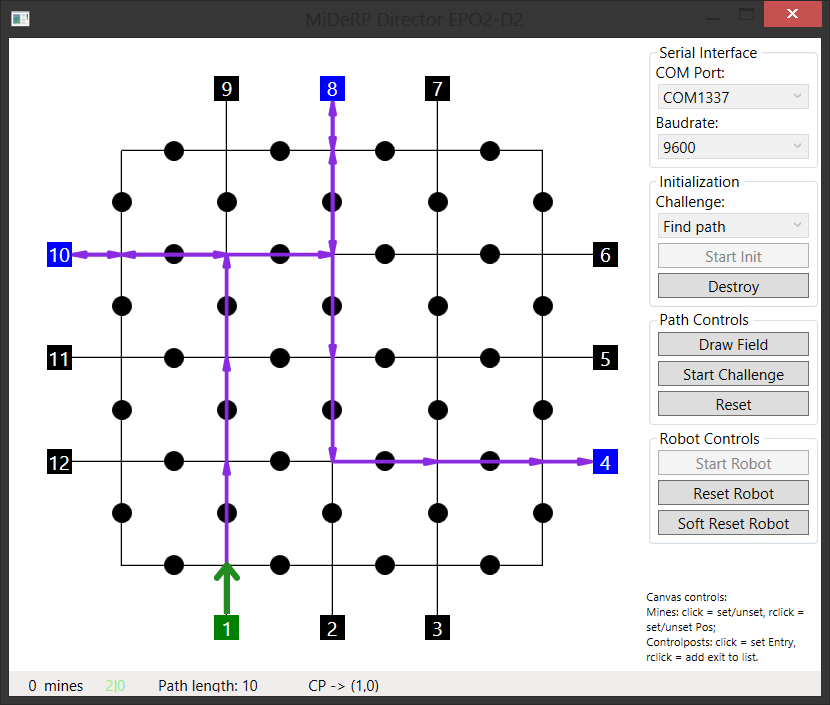
\includegraphics[width=0.95\textwidth]{resource/director-initial-screenshot}
		\caption{Een voorbeeld van de interface bij een willekeurig berekend pad, de robot heeft nog niet bewogen en gaat naar 10, 8 en 4}
		\label{fig:director-initial}
	\end{subfigure}
	\begin{subfigure}{0.48\textwidth}
		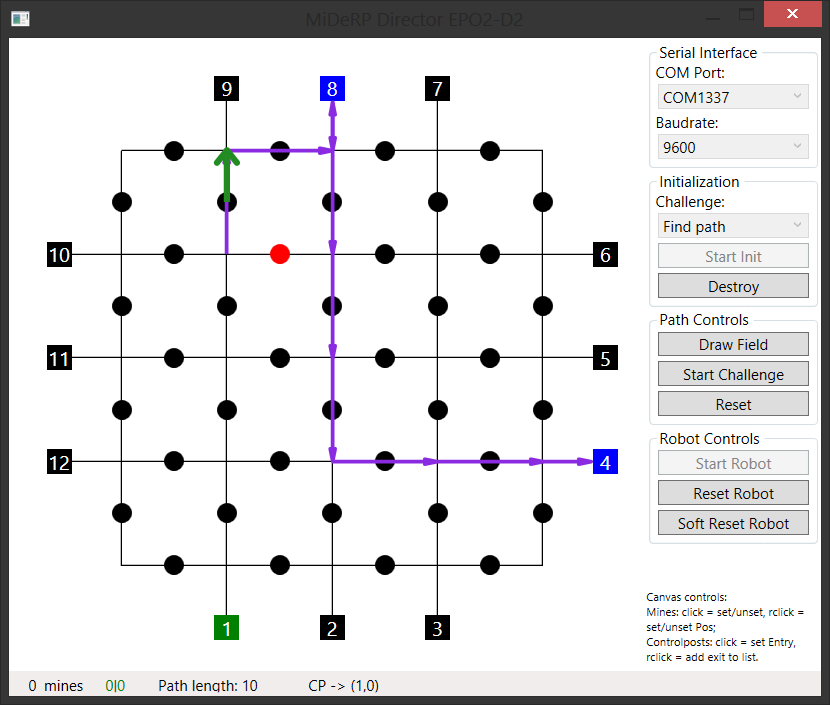
\includegraphics[width=0.95\textwidth]{resource/director-ontheway-screenshot}
		\caption{Een voorbeeld van de interface bij een willekeurig berekend pad wanneer de robot al enige tijd onderweg is en een mijn is tegengekomen}
		\label{fig:director-ontheway}
	\end{subfigure}
	\caption{Twee schermafdrukken dan de Director in actie.}
	\label{fig:director}
\end{figure}

\subsection{Navigatie}
Om de A* implementatie te gebruiken was er een "brug" nodig tussen de managed omgeving en de unmanaged omgeving.
Omdat deze heel erg verschillen moeten er speciale functies geschreven worden zodat de unmanaged code aangeroepen kan worden en data uitgewisseld.
Wij hebben dit gedaan via Interop (voor de functie aanroepen [DllImport]) en de Marshaller (voor de equivalenten van malloc en free).
\subsection{Communicatie}
De communicatie met de XBee module verloopt via een seriële poort. Deze is gemakkelijk te gebruiken in .NET. Er is een event waar men zich op kan abonneren om zo op de hoogte gesteld te worden als er data gearriveerd is. Wij hebben een protocol gemaakt om de communicatie tussen de controller en de robot te bewerkstelligen. (zie sectie \ref{sec:communicatie} voor de specificaties)

\subsection{Controller}
De controller regelt de reacties op de seriële events, deze krijgt dus een byte binnen vanuit de robot. Bijvoorbeeld een "Enquiry" (Waar moet ik heen), de controller gaat dan kijken waar hij denkt dat de robot is en wat de volgende actie zou moeten zijn om het pad te volgen.
Dit stuurt hij dan terug naar de robot, zodat deze weer verder kan rijden.

Als de controller van mening is dat we aangekomen zijn op het punt van bestemming stuurt die een "Done" naar de robot. Deze stopt dan aan het eind van de lijn.
Zo ook als de robot een mijn detecteert en de PC ontvangt deze dan wordt deze aan de lijst met mijnen toegevoegd en naar het unmanaged geheugen gekopieerd, zodat er een nieuw pad berekend kan worden.
In de tussentijd is de robot dan al weer teruggereden naar het kruispunt en vraagt hij, daar aangekomen, weer welke richting hij moet nemen.

Zo worden alle control points die geselecteerd waren afgereisd.

\subsection{Gebruikersinterface en visualisatie}
De gebruikersinterface is opgebouwd uit twee onderdelen, een plattegrond en de besturing.
De besturing bevat knoppen voor functies als verbinden met de XBee module het initialiseren het het selecteren van de challenge.
De plattegrond wordt getekend door middel van een canvas element, hierop kan met vormen, zoals cirkels en lijnen, getekend worden. We hebben een klasse voor een pijl moeten maken omdat deze niet aanwezig was in WPF.
De plattegrond word live geupdate met informatie die binnen komt op de seriële poort, de pijl die de positie van de robot aangeeft verschuift dan ook realtime en mijnen zullen ook verschijnen.
Er kan op de control posts geklikt worden om deze aan te wijzen als te bezoeken of als start aan te geven.
De mijnen kunnen geplaatst en weer verwijderd worden.

\end{document}